\documentclass{sig-alternate}


\usepackage{latexsym}
\usepackage{amsmath}
\usepackage{color}
\usepackage{graphicx}
\usepackage{amssymb}
\usepackage{epstopdf}
\usepackage{algorithmic}
\DeclareGraphicsRule{.tif}{png}{.png}{`convert #1 `dirname #1`/`basename #1 .tif`.png}



\def\punto{$\hspace*{\fill}\Box$}
\newcommand{\nop}[1]{}
\newcommand{\tuple}[1]{{\langle#1\rangle}}
\def\lBrack{\lbrack\!\lbrack}
\def\rBrack{\rbrack\!\rbrack}
\newcommand{\Bracks}[1]{\lBrack#1\rBrack}


\newtheorem{theorem}{Theorem}[section]
\newtheorem{proposition}[theorem]{Proposition}


\nop{
\newtheorem{metatheorem}{Metatheorem}[section]
\newtheorem{example}[theorem]{Example}
\newtheorem{algorithm}[theorem]{Algorithm}
\newtheorem{definition}[theorem]{Definition}
\newtheorem{property}[theorem]{Property}
\newtheorem{corollary}[theorem]{Corollary}
\newtheorem{lemma}[theorem]{Lemma}
\newtheorem{remark}[theorem]{Remark}
\newtheorem{conjecture}[theorem]{Conjecture}
\newtheorem{proviso}[theorem]{Proviso}
\newtheorem{todo}[theorem]{ToDo}
} % end nop



\conferenceinfo{SIGMOD}{'10 Indianapolis, IN}


\title{The Cumulus System for Exact
%, Low-Latency
Online Aggregation in the Cloud}


%\title{Streamlining Data Warehousing through Compilation}
\numberofauthors{3}
\author{}%Oliver Kennedy, Yanif Ahmad, Christoph Koch}
%\date{}                                           % Activate to display a given date or no date

\toappear{}

\newtheorem{example}{Example}

\begin{document}

\maketitle
%\section{}
%\subsection{}

\abstract{
In this paper we present Cumulus, a compiler for producing customized data warehouses.  Cumulus uses a novel set of techniques to compile the execution of complex queries down to simple message-passing operations between a set of map datastructures.  By expressing the query result in terms of a recursively defined view-maintenence problem, the data warehouse is able to maintain a set of intermediate results that make it possible to incrementally update the data warehouse in realtime.  The intermediate results produced by these incremental updates can also be used to simplify processing of OLAP-style queries.  Furthermore, the ease of partitioning and distributing Cumulus' map datastructures makes it feasible to deploy the entire data warehouse in-memory.  The result is a power-efficient data warehousing infrastructure that can maintain synchronization with a relational database, allowing online processing of high-volume aggregate queries.
}



It is immediately plausible that one can do better than re-evaluate a query from scratch whenever the database changes a little. Incremental view maintenance (IVM) capitalizes on this insight \cite{DBLP:journals/tods/BunemanC79,DBLP:conf/sigmod/ShmueliI84,DBLP:conf/sigmod/BlakeleyLT86,roussopoulos-tods:91,DBLP:conf/vldb/CeriW91,DBLP:conf/deductive/GuptaKM92,DBLP:conf/sigmod/GuptaMS93,griffin-sigmod:95,yan-vldb:95,colby-sigmod:96,GHJ1996,kotidis-tods:01}. It is a solid, settled technique that has been implemented in many commercial DBMS, but has seen little new research activity in recent years and has gathered a little dust.

Now there is an exciting and potentially game-changing new development \cite{ahmad-vldb:09, koch-pods:10, kennedy-ahmad-koch-cidr:11}, an extreme form of IVM where all query evaluation work reduces to adding data (updates or materialized query results) to other materialized query results.  No join processing or anything semantically equivalent happens at any stage of processing. This works for a fragment of SQL with equijoins and aggregation, but without inequality joins or nesting aggregates.


Let us digest this, because the last claim goes counter to query processing intuitions to the point of absurdity. The main idea is the following: Classical IVM revolves around the idea that a materialized view can be maintained under updates by evaluating a so-called delta query and adding its result to the materialized view. The delta query captures how the query result changes in response to a change in the database. The new observation is that the delta query can be materialized and incrementally maintained using the same idea, making use of a delta query to the delta query, which again can be materialized and incrementally maintained, and so on, recursively. This works for classes of queries whose deltas are in some way structurally simpler than the base queries (e.g. having fewer joins), allowing this recursive query transformation to terminate. (It does so with a final trivial $k$-th delta query that does not refer to the database at all.) Termination is ensured for select-project-join queries with certain forms of aggregation, but some other features of SQL (specifically aggregations nested in where-conditions) have to be excluded. 

So where do the joins go? They {\em really} go away, as a benefit of incremental computation. If we want to compute $(x+1)*y$ and know $x*y$ and $y$, we only need to add $y$ to $x*y$, and the multiplication goes away. This is what happens when incrementally maintaining a join, where the join takes the place of multiplication. The pattern just sketched in basic algebra is not just an intuition but exactly what happens, and \cite{koch-pods:10} develops the algebraic framework to formalize this. We observe that the symbol 1 above represents the update workload.  In the incremental query processing framework, it must be a {\em constant} number of tuples that are changed in each incrementation step.

\comment{
To the reader who still cannot accept that joins can be replaced by no joins, we observe that the history of all incremental updates to the materialized view taken together is still essentially an execution of a nested loops join, that is, overall the value $x*y$ is constructed by adding $x$ copies of $y$. So if we put all the work associated with the individual updates happening over time together, the join work is still done. But refreshing the view in response to a single update does not require joins.
}

On paper, this approach clearly dominates classical IVM: if classical IVM is a good idea, then doing it recursively is an even better idea: The same efficiency-improvement argument for incremental maintenance of the base query also applies to the delta query. Argued from the viewpoint that joins are expensive and this approach eliminates them, one should expect a potential for excellent query performance.

But does this expectation translate into real performance gains? A priori, the cost of the bulk addition of materialized views or the costs associated with storing and managing additional auxiliary materialized views (for delta queries) might be more considerable than expected.


\medskip


This paper presents the lessons learned in an effort to realize recursive IVM, spanning nearly three years of intense work, to generalize it to be applicable on all or most of SQL, and to understand its strengths and drawbacks.
The contributions of this paper are as follows.
\begin{itemize}
\item
Multilevel IVM bears the promise of providing materialized views of complex SQL queries, without
window semantics or other restrictions, at very high refresh rates. We start by showing that there is
a need for such functionality, creating a benchmark consisting of automated trading and ETL workloads.
We show that state of the art systems cannot deliver materialized views refreshed at the rates
that some application domains (algorithmic trading, real-time analytics) require.
This is the challenge we set ourselves for the techniques and system described in this paper.

\item
We develop the vision of multilevel IVM further into a workable system.
While the techniques of \cite{ahmad-vldb:09, koch-pods:10} as well as existing implementations of
IVM in commercial DBMS are very restricted and exclude nested queries and other features of SQL,
we create the machinery to perform IVM and even recursive IVM on most of SQL (with the exception of
support for null values). To do this, we generalize the techniques of \cite{ahmad-vldb:09, koch-pods:10}
to not always materialize full delta queries but instead subexpressions that allow us to perform
IVM and maximize the performance obtained. This leads us to a query optimizer in which
the materialization of subqueries is a degree of freedom in optimization, and can be applied anywhere
in the input query or the delta queries obtained by applying this optimization.

To put ourselves in the position of using such an optimizer, we have to create suitable
intermediate representations of queries that support binding patterns for sideways information
passing, we study when and how to efficiently initialize views, and present query decomposition
and factorization techniques that lead to efficient formulations of update triggers that refresh our
views.

\item
Once high-level trigger programs for refreshing views based on multilevel IVM have been created,
we compile them further into highly efficient machine code.
We present our techniques for achieving this, which make use of sophisticated deforestation and
fusion techniques from the compilers literature.

\item
We have implemented our compiler and performed extensive experimentation with it. Our experiments
indicate that frequently, particularly for queries that consist of many joins of nested aggregation
subqueries that are not correlated through subqueries, our compilation approach dominates the
state of the art, often by multiple orders of magnitude. There are also queries in our benchmark
on which our techniques do not fare well; these usually involve the creation and maintenance of huge
auxiliary views whose data is rarely used by other views. These scenarios could be much improved upon
by suitable garbage collection strategies on auxiliary views. This is future work, and we consider
it likely that once such a technique has been integrated into our compiler, it will outperform the
state-of-the-art on an even wider range of queries.
\end{itemize}


The structure of the paper follows the order of contribution just laid out.















\comment{
This paper presents the lessons learned in an effort to realize aggressive IVM as motivated above. It represents an effort spanning nearly three years of intense work, which demonstrates that there are considerable technical challenges to be resolved. These key challenges are described next.


{\bf Compilation of update trigger code.}
%
The work that has to take place to update one materialized view with another (i.e., an auxiliary view representing a delta) is conceptually very simple; it essentially consists of bulk-adding tuple multiplicities of one view to another.

This updating work to be performed is particularly well-behaved and can be exploited for efficient evaluation:
\comment{
As observed in \cite{koch-pods:10}, this work is highly data-parallel. While parallel query evaluation is not the focus of the present paper, the updating work to be performed is particularly well-behaved. This can be exploited for efficient evaluation:
}
Classical query engines employ interpretation and large-gra\-nu\-la\-ri\-ty query operators such as joins to execute query plans.
In the past, IVM has used such query engines to evaluate its delta queries.
Instead, it is natural to avoid both query operators and plan interpretation, and the conceptual simplicity of the required work calls for aggressive code inlining and the elimination of the usual overheads due to interpreted query evaluation. It leads us to the compilation of view refreshing to lightweight machine code.

A considerable challenge is to determine suitable intermediate representations of query expressions to be used in the compiler. Such expressions in general have complex binding patterns which represent information flow. In general, this flow is not exclusively bottom-up.
Examples include complex conditions and nested subqueries correlated with their superqueries. Such expressions have input variables, and can only be evaluated if values for these input variables are given. In general, such expressions have to be materialized, which causes difficulties: how to determine a suitable domain for these input variables for which to materialize the results of the expressions, how to represent and store such materialized structures, and how to dynamically maintain the domains of input variables as updates add previously unseen values.


{\bf Compiler optimizations.}
%
Naively materializing delta queries, their delta queries, and so on causes the materialized views of the higher deltas to have high arity: in fact, the dimensionality can be as high as the arity of the product of all the relations joined together in the input query. The resulting size of the materialized views is of course unacceptable. As observed earlier \cite{ahmad-vldb:09, koch-pods:10} though, the materialized views can be losslessly decomposed into small views: taking a delta each time eliminates some join constraints, turning the views indeed into products.

This calls for factorization and decomposition techniques without which this approach would not be workable. In turn, however, recursive decomposition of delta queries of the various trigger programs (for insertions into and deletions from the relations occurring in the query) may produce large numbers of highly redundant factor views. This makes it essential to aggressively perform common subexpression elimination as well as deforestation and fusion techniques from the compiler literature.

In our implementation and experimentation efforts, this turned out to be much more important for satisfactory performance of the system than expected: without these techniques, recursive compilation for IVM with factorization as described in \cite{koch-pods:10} can result in hundreds of views to be maintained for a large join query, most of which are redundant and can be eliminated.
\comment{
Common subexpression elimination has been studied in the context of multi-query optimization, but here it takes a much more central role: without it, query performance will deteriorate by orders of magnitude almost every time: This is true even though we are referring to the compilation products of a single query, not a workload of multiple queries whose naturalness, if the queries share many subqueries, is often debatable. Thus, optimizations which are typically associated with compilers for general-purpose programming languages rather than query optimizers take a central role.
}
\comment{
We have also learned that some of the natural optimizations used in compilers for general-purpose programming languages rather than query optimizers take a central role. In particular, certain types of common subexpression elimination, loop fusion and analogous deforestation techniques for aggregations, are key to obtaining acceptable performance.
}
However, several of these optimizations such as deforestation have no form of expression in high-level query plan formalisms used in classical query optimization or recursive IVM. Thus, more than one internal intermediate representation (IR) of code is necessary.

\comment{
Our experiences led to two functional followed by one imperative IR. The functional IRs are a cleaned-up form of the algebraic expressions based on rings of queries and databases from \cite{koch-pods:10}, followed by a lower-level, Haskell-like and nearly general functional programming language in which we perform further forms of fusion and deforestation. The imperative IR is used in the compiler backend before imperative code generation. \comment{It is used for further optimizations that cannot be naturally expressed in a functional IR.} Overall, this leads us to a multi-stage reference compiler architecture for optimizing compilation of database queries to imperative code that we believe is general and relevant outside the context of incremental computation (cf. also Delite \cite{delite:11}).
}


\comment{
{\bf Side effects and initial value computation.}
%
Recursive IVM creates challenges we have not seen sufficient study of before, although they occur in simpler form in previous data management architectures that combine updating with querying, such as OLTP systems and stream processors: It is the tension between the convenience of viewing queries as pure functions of the data, and the {\em side-effects} that are updates.
In recursive IVM, an update triggers a variety of computations -- queries -- on various levels of a hierarchy of materialized views; one such computation creates data that is stored and used by another. These interleaved computations conceptually are meant to happen together, and side-effects must be carefully orchestrated to ensure a consistent database state after each update.

\comment{
In the context of recursive IVM, an update triggers a variety of computations -- queries -- on various levels of a hierarchy of materialized views; one such computation creates data that is stored and used by another. Compared to active databases, where certain events can trigger a cascade of computations, in the context of recursive IVM we face additional challenges in that interrelated computations do not profit from the benefits of isolation and conceptual serialization due to transaction semantics. The interleaved computations conceptually are meant to happen together.
}

As mentioned above, we in general need to materialize query expressions with binding patterns: queries that have input variables whose values cannot be determined from the query itself. The dynamic extension of the domains of these input variables and the resulting augmentation of the materialized views requires special initialization code distinct from the incrementation code (the compiled delta queries); this adds additional subtle challenges to the compilation framework. Most importantly, deciding how the domains of input variables of a materialized view has to be extended and optimizing the resulting code requires an intricate analysis of side effects across the hierarchy of materialized views.
} % end comment


{\bf Extraction/materialization as a first-class citizen of query optimizers.}
%
As stated above, the framework of recursive IVM requires delta queries to be structurally simpler than the queries they are deltas to. This is not the case for full SQL. This calls for abstracting from the strict notion of recursive IVM discussed in \cite{ahmad-vldb:09, koch-pods:10}. The key rewriting is to extract and materialize a subquery for IVM. This rewriting can be performed at multiple places in the query, as well as in delta queries that are used to incrementally maintain the materialization. In \cite{ahmad-vldb:09, koch-pods:10} the extracted subquery is always the full query or a factor in its product decomposition. But this is really an arbitrary restriction which can be lifted without causing fundamental problems.

This turns our compilation task into one of generating query evaluation code using an optimizer that has an {\em extract/materialize operator} that can be applied anywhere in the query, subject to optimization decisions (which we know from the literature on answering queries using views) but which also further compiles the delta queries auxiliary to materialization.


\medskip

The structure of the paper is as follows. Next, in Section~\ref{sec:sota}, we provide further motivation for the study of multilevel IVM by demonstrating by experimentation that low-latency continuous queries from ETL, monitoring and computational finance cannot be easily expressed by or managed by classical stream processors, or any other kind of existing engine. 
In Section~\ref{sec:compiler}, we present our compilation approach in detail, covering the various stages of a compiler from multilevel
incremental view maintenance to code generation.
Section~\ref{sec:experiments} returns to experimentation, picking up where we left off at the end of Section~\ref{sec:sota}, with all current data management systems failing to provide satisfactory performance for frequently fresh views for the workload proposed there.
We conclude with Section~\ref{sec:conclusion}.
} % end comment






\section{Compilation to M3}
\label{sec:compiler}


\subsection{Query Calculus}


\def\safe{\mbox{safe}}
\def\AggSum{\mbox{Sum}}

Our calculus consists of
{\em formulae} of positive quantifier-free relational domain calculus
(i.e., formulae constructed from conjunctions ``and'',
disjunctions ``or'', and atoms) and of {\em terms}.
%
The atomic formulae are {\em true}, {\em false}, relational atoms $R(\vec{x})$
where $\vec{x}$ is a tuple of variables,
and atomic constraints of the form $t_1 \;\theta\; t_2$ comparing two terms
$t_1$ and $t_2$ using comparison operations $\theta$ of $=$, $\neq$, $<$,
and $\leq$.
%
Terms are built from variables, constants, built-in function calls
$f(\vec{t})$, where $\vec{t}$ is a tuple of terms,
and aggregrate sums ($\AggSum$) using addition and multiplication.
Built-in functions compute their result entirely based on their input
terms, not accessing the database (e.g., mod or string concatenation).
In short, the grammar for formulae $\phi$ and terms $t$
(given variables $x$, constants $c$, relation names $R$,
comparison operators $\theta$,
and builtin functions $f$) is
\begin{eqnarray*}
  \phi &\mbox{::-}& \phi \land \phi
               \mid \phi \lor \phi \mid (\phi)
               \mid \mbox{true} \mid \mbox{false} \mid R([x(,x)^*])
               \mid t \;\theta\; t
\\
  t &\mbox{::-}& t * t \mid t + t \mid (t) \mid c \mid x \mid f([t(,t)^*]) \mid
                 \AggSum(t, \phi)
\end{eqnarray*}

An aggregate term $\AggSum(t, \phi)$
is {\em constraints-only} if $\phi$ does not
contain relational atoms $R(\vec{x})$ (but atomic constraints $s \theta t$).
We can also think of such an aggregate term as a (functional)
if-statement (if $\phi$ then t else 0)
or, using C syntax, ($\phi$ ? $t$ : 0).

We will make one important syntactic restriction, namely that
no $\AggSum$ terms may occur in atomic constraints.

Formulas and terms are evaluated relative to a given set of
{\em bound variables}.
The bound variables of a subformula are the bound variables of the formula.

Given a set of bound variables $B$,
the {\em safe variables} of a formula are defined bottom-up
as usual in relational
calculus (see e.g. \cite{DBLP:books/aw/AbiteboulHV95}). In particular,
\begin{eqnarray*}
\safe_B(R(\vec{x})) &:=& \{x_i\} \cup B \\
\safe_B(\phi \land \psi) &:=& \safe_B(\phi) \cup \safe_B(\psi) \\
\safe_B(\phi \lor \psi)  &:=& \safe_B(\phi) \cap \safe_B(\psi) \\
\safe_B(\phi \land x = y) &:=&
\left\{\begin{array}{ll}
\safe_B(\phi) \cup \{ x, y \} &\dots
\mbox{$x$ or $y$ is} \\
&\;\;\; \mbox{in $\safe_B(\phi)$} \\[.5ex]
\safe_B(\phi) &\dots \mbox{otherwise}.
\end{array} \right.
\end{eqnarray*}
Here $\{x_i\}$ drops order and turns the tuple $\vec{x}$ into a set.

Given a term $\AggSum(t, \phi)$ with bound variables $B$,
the bound variables of $\phi$ are $B$ and the bound variables of $t$ are
the safe variables of $\phi$, $\safe_B(\phi)$.
The bound variables of a subterm are the bound variables of the term.
Variables occuring as terms must be bound.

\begin{example}\em
Given singleton bound variable set $\{ y \}$,
\[ \AggSum(u * f(z), \underbrace{(\underbrace{(\underbrace{R(x, z)}_{x,y,z} \lor \underbrace{y=z}_{y,z})}_{y,z} \land z = w)}_{y,z,w}) \]
is invalid: The safe variables of the formula are
$\{y,z,w\}$, so $u$ is not bound in the term $u * f(z)$. The overall term
becomes valid for bound variables $\{u,y\}$.
\punto
\end{example}


\def\db{{\cal{A}}}

The semantics of formulas and terms is given by a (polymorphic) function
$\Bracks{\cdot}(\cdot, \cdot)$ that takes a database and values for the
bound variables as arguments. Given database $\db$ and values $\vec{b}$ for
the bound variables,
$\Bracks{\phi}(\db, \vec{b})$ evaluates to a relation and
$\Bracks{t}(\db, \vec{b})$ evaluates to a value of the type of
terms.\footnote{In practice,
we have several types such as integers and floats, but
here we will not talk about types and will assume that all terms evaluate to,
say, floating point numbers. However, our implementation supports the
main data types of SQL, and no noteworthy observations were made achieving
this.}
We assume a multiset semantics for relations, which is important to note
since we focus on computing aggregates. The multiset semantics of formulas
is defined by their well-known translation to relational algebra
(Codd's theorem), and the standard multi-set semantics of
(in our case, positive) relational algebra. 
$\AggSum$ terms are new, but otherwise the
semantics of terms is obvious.
A term $\AggSum(t, \phi)$
computes the sum of the values $t[\vec{x}]$
over the distinct valuations (with duplicates)
of the safe variables $\vec{x}$ of $\phi$, i.e.,
given a database $\db$ and values $\vec{b}$ for the bound variables of $\phi$,
\[
\Bracks{\AggSum(t, \phi)}(\db, \vec{b}) =
\sum_{\vec{v} \;\mathrm{in}\; \Bracks{\phi}(\db, \vec{b})} \Bracks{t}(\db, \vec{v}).
\]


{\bf From SQL to the Calculus}.
Given our semantics definition, the translation from SQL to our calculus is
straightforward.
%
%We focus on aggregation queries, specifically
%sum aggregation queries (count and avg aggregation queries can be encoded
%using sum). Aggregates can be nested in the SELECT clause, but not in
%the FROM, WHERE, or HAVING clause. We support GROUP by, although in a way
%that may at first seem nonstandard. We do not support DISTINCT.
%
A SQL aggregate query
\begin{verbatim}
SELECT groupcols, SUM(t)
FROM   R1 r11, R1 r12, ..., R2 r21, ...
WHERE  cond
GROUP BY groupcols
\end{verbatim}
is expressed in the calculus as
\[
\AggSum(t, R_1(\vec{x}_{11}) \land R_1(\vec{x}_{12}) \land \dots
\land R_2(\vec{x}_{21}) \land \dots \land \mbox{cond})
\]
with {\em bound variables} groupcols.


\begin{example}\em
\label{ex:self-join-calc}
The query of Example~\ref{ex:self-join} translates to
$\AggSum(1, \mbox{Customer}(c_1,n_1) \land \mbox{Customer}(c_2, n_2) \land
n_1=n_2)$ in the calculus, with bound variable $c_1$.
\punto
\end{example}

\subsection{Normalization and Simplification}


A semiring is an algebra with two associative operations,
$+$ and $*$, that
have neutral elements (called 0 and 1, respectively), which satisfy
distributivity ($a*(b+c)= a*b + a*c$), and where $+$ is commutative.
Semirings with variables
have polynomials, that is, each expression of the
semiring can be mapped to an equivalent expression that is
a sum of flat products (the products are also known as {\em monomials}\/).
Turning semiring expressions into polynomials just means to apply
distributivity repeatedly until we end up with a polynomial.
This can be combined with simplification operations based on the 1 and
0-elements, i.e., $\alpha * 1$ maps to $\alpha$, $\alpha*0$ maps to $0$, and
$\alpha+0$ maps to $\alpha$. Polynomials can be conveniently implemented
as lists of lists of atoms, where an empty top-level list (i.e., polynomial)
has value 0 and an empty monomial list has value 1.

Both our formulae and our terms are semirings; in particular,
in the semiring of formulae, $\land$ is the product operation,
$\lor$ is addition,
and $\textit{false}$ and $\textit{true}$ are 0 and 1, respectively.

For arbitrary terms $s$ and $t$ and formulas $\phi$ and $\psi$,
$\AggSum$ terms can be simplified using the following equations (to be
applied by replacing a left by a right hand side expression)
\begin{eqnarray*}
\AggSum(t, \textit{true}) &=& t \\
\AggSum(t, \textit{false}) &=& 0 \\
\AggSum(0, \phi) &=& 0 \\
\AggSum(s+t, \phi) &=& \AggSum(s, \phi) + \AggSum(t, \phi) \\
\AggSum(t, \phi \lor \psi) &=& \AggSum(t, \phi) + \AggSum(t, \psi)
\end{eqnarray*}

All these algebraic laws can be applied, and the calculus expression
be maximally simplified, in a single bottom-up pass of the expression.
A term ($\AggSum$ or other) maximally simplified in this way
is a sum of terms that contain neither $+$ nor $\lor$; we call such 
normalized terms {\em recursively monomial}.
Define function RecMonomials to compute the list of recursively monomials
of a term.

\def\vars{\mbox{vars}}

{\bf Factorization of monomial aggregate terms}.
For $e$ either a formula or a term, let $\vars(e)$
be the set of all variables occurring in $e$.
Factorization employs the equivalence
\[
\AggSum(s*t, \phi \land \psi) = \AggSum(s, \phi) * \AggSum(t, \psi)
\]
which is true if
$(\vars(s) \cup \vars(\phi)) \cap (\vars(t) \cup \vars(\psi)) = \emptyset$.

Consider an aggregate term $\AggSum(t, \phi)$ where both $t$ and $\phi$ are
monomials, consisting of the sets $T$ and $F$ of atomic terms and formulae,
respectively (that is, $t = \prod T$ and $\phi = \bigwedge F$).
We can think of the
elements of the two-sorted set $T \cup F$ as the hyperedges of a
{\em hypergraph},
where the function $\vars(e)$ maps hyperedge $e$ to the nodes that are
part of it.
The set of {\em connected components} ${\cal C}$ of this hypergraph is the
maximum cardinality set of subsets of $T \cup F$ such that for any
two components $C_1, C_2 \in {\cal C}$ with $C_1 \neq C_2$,
$\vars(C_1) \cap \vars(C_2) = \emptyset$. Asking for the maximum number of
nonoverlapping components is of course the same as asking for components of
minimum size, and the set of connected components is unique and can be computed
in linear time using Tarjan's algorithm. Given ${\cal C}$, each component
$C \in {\cal C}$ can again be partitioned by sort into a monomial term $t_C$
and a monomial formula $\phi_C$.
%
% By convention, if $C$ does not contain atomic terms, $t_C = 1$ and if $C$
% does not contain atomic formulae, $\phi_C = \textit{true}$. It is not
% difficult to verify that
%
$\AggSum(t, \phi)$ is equivalent to
\[
\prod_{C \in {\cal C}} \AggSum(t_C, \phi_C).
\]

{\em Recursive factorization}, given term $\AggSum(t, \phi)$, first recursively
factorizes the aggregate terms in $t$ before applying factorization as
just described on the top level.


\begin{example}\em
The connected components of term
\[
\AggSum(5 * x * \AggSum(1, R(y, z)) * w, R(x,y) \land S(z) \land R(v, w))
\]
are
$\{ \{5\}, \{ x, R(x,y), \AggSum(1, R(y, z)), S(z) \}$,
$\{ w, R(v, w)) \} \}$
and thus the term factorizes as
$\AggSum(5, \textit{true}) *
\AggSum(x * \AggSum(1$, $R(y, z)), R(x, y) \land S(z)) *
\AggSum(w, R(v, w)))$.
$\AggSum(5, \textit{true})$ simplifies to $5$.
\punto
\end{example}


{\bf Variable elimination}.
Given an abitrary monomial formula $\phi = \bigwedge (E \cup O)$,
where $E$ is the set of equality
atoms $x=y$ and $O$ is the set of remaining atoms (either set may be empty),
and a set of bound variables $B$.
We eliminate redundant variables as follows.

Consider the equivalence classes of the equivalence relation $E$.
For each equivalence class $C$ of $E$, distinguish an element
(i.e., variable) as $x_C$ such that,
if $B \cap C \neq \emptyset$, $x_C$ is an arbitrary element of $B \cap C$;
otherwise, it is an arbitrary element of $C$.
Create a unification mapping
$\Theta$ that maps each unbound variable $y$ of $E$ to $x_{[y]}$ (where $[y]$ is the
equivalence class of $y$) and is the identity on the bound variables.
Now substitute all variables in $O$
using $\Theta$, obtaining $O'$. Let
$E' =  \bigcup \{ y = x_{[y]} | y \in ((B \cap [y]) -  x_{[y]}) \}$.
Then we replace $\phi$ by $(\bigwedge O') \land \bigwedge E'$.

Given a term $\AggSum(t,\phi)$ where $\phi$ is a monomial,
and bound variables, we eliminate variables by 
first eliminating variables in $\phi$, creating $\phi'$ and $\Theta$.
Then we substitute all variables of $t$ that are in the domain of $\Theta$
using $\Theta$, obtaining $t'$. The result, $\AggSum(t', \phi')$, is equivalent
to $\AggSum(t,\phi)$.


\begin{example} \em
Given term $\AggSum(y*v*r, R(z, v) \land v<q
\land x=y \land x=z \land u=v \land v=w \land q=r)$
and bound variables $\{x,y,z,r\}$.
The variable equivalence classes are
$\{ \{x,y,z\}, \{u,v,w\}, \{q,r\} \}$. We choose the rightmost variable in
each class as the variable to substitute by. In the first class, we can choose
freely because all members are bound. In the second we can choose freely
because none are bound. In the third, we must choose $r$ because it is bound
and $q$ is not.
The mapping is
$\Theta = \{ x \mapsto x, y \mapsto y, z \mapsto z, u \mapsto w, v \mapsto w,
w \mapsto w, q \mapsto r, r \mapsto r \}$.
We apply $\Theta$ to $y*v*r$ and $R(z, v) \land v < q$ and obtain
$z*w*r$ and $R(z,w) \land w<r$, respectively. The simplified
overall term is
$\AggSum(z*w*r, R(z,w) \land w<r \land x=z \land y=z)$.
\punto
\end{example}


{\bf Extraction of aggregates}.
For a term $t$ and its set $B$ of bound variables,
the function ExtractAggregates($t$, $B$)
replaces each maximal subterm $s$ of $t$
that is of the form $\AggSum(\cdot, \cdot)$ but is not constraints-only
by a ``map access''  $m[\vec{x}]$, where
$m$ is a new name and $\vec{x}$ is the set of variables
both bound at $s$ and used in $s$ ordered arbitrarily.
The result of ExtractAggregates thus is a pair $(t', \Theta)$ of the remainder
term $t'$ and a mapping $\Theta$ from map accesses $m[\vec{x}]$ to extracted
subterms $s$ (which could be used to undo the extraction).

\begin{example}\em
Let $t$ be the term
\begin{multline*}
\AggSum(x*\AggSum(w, R(v, w), R(w, z)), x<y \land y=z) \\
*\; 5 * y * \AggSum(u, R(u, x)).
\end{multline*}
Then ExtractAggregates($t$, $\{x,y\}$) returns the pair consisting of term
$\AggSum(x*m_1[z], x<y \land y=z) * 5 * y * m_2[x]$
and the mapping
$\{
m_1[z] \mapsto \AggSum(w, R(v, w), R(w, z));
m_2[x] \mapsto \AggSum(u, R(u, x))
\}$.
\punto
\end{example}


{\bf Lifting ifs}. Observe that if $\phi$ is a constraints-only term in which
all variables are bound, then
\begin{eqnarray*}
\AggSum(t, \phi \land \psi) &=& \AggSum(\AggSum(t, \psi), \phi) \\
t * \AggSum(t', \phi) &=& \AggSum(t * t', \phi)
\end{eqnarray*}
Thus, given a recursively monomial term, we can lift $\phi$ to the top. 
Let function LiftIfs do exactly this.

\begin{example}\em
This will be used in Example~\ref{ex:self-join-compile}:
\begin{multline*}
\mbox{LiftIfs}((-1) * \AggSum(1, C(c_2, n) \land c_1=c), \{c_1, c, n\}) = \\
\AggSum((-1) * \AggSum(1, C(c_2, n)), c_1=c).
\end{multline*}
\end{example}


Given a recursively monomial term $t$ and a set of bound variables $B$,
let the function Simplify($t$, $B$) recursively factorize $t$, then perform
variable elimination, and finally if-lifting.


\subsection{Delta Computation}


\def\dt{\Delta_{\pm R(\vec{t})}}


Given a term or formula $\alpha$
of our calculus, and an insertion or deletion of a
single tuple $\vec{t}$ to/from a relation $R$ of the database.
We denote the database obtained from database $\db$ by this update by
$\db \pm R(\vec{t})$.
We can express a delta $\Delta_{\pm R(\vec{t})} \alpha$
(which is a term if $\alpha$ is a term and a formula if $\alpha$ is a formula)
such that,
given current database $\db$ and values $\vec{b}$ for the bound variables,
\begin{eqnarray}
\Bracks{\alpha}(\db \pm R(\vec{t}), \vec{b}) &=&
\,\Bracks{\alpha}(\db, \vec{b}) \pm \,\Bracks{\dt \alpha}(\db, \vec{b}).
\label{eq:delta}
\end{eqnarray}

The delta rules for semirings are as follows. We use $+$ and $*$ for the
addition and multiplication operations; for formulae, these are of course
$\lor$ and $\land$, respectively.
\[\begin{array}{lllcr}
\dt (\alpha + \beta) &:=& ((\dt \alpha)    &+& (\dt \beta))
\\[1ex]
\dt (\alpha \,*\, \beta)
   &:=& ((\dt \alpha)               &*& \beta\;\,) \\
   &+ & (\quad\quad\quad\;\, \alpha &*& (\dt \beta)) \\
   &+ & ((\dt \alpha)               &*& (\dt \beta))
\end{array}\]

For atomic formulae and terms,
\[\begin{array}{lllr}
\dt \AggSum(t, \phi)
   &:=& \AggSum((\dt t), & \phi\;\,) \\
   &+ & \AggSum(\quad\quad\quad\; \,t,  & (\dt \phi)) \\
   &+ & \AggSum((\dt t), & (\dt \phi))
\\[1ex]
\dt R(x_1, \dots, x_k) &:=& \big( \bigwedge_{i=1}^k (x_i = t_i) \big)^\pm
\end{array}\]
and, for $S$ a relation different from $R$,
\[
\dt S(x_1, \dots, x_l) := \textit{false}.
\]
For all other atomic terms and formulae, $\dt$ is the zero-element
of their respective semirings (that is, $0$ and $\textit{false}$,
respectively.)

Here $(\cdot)^\pm$ is an annotation that we do not give a formal semantics
to for space limitations, but explain how to eliminate. $\phi^+$ is just
$\phi$ and $\phi^-$ intuitively defines a relation of ``negative'' tuples.
We define $\phi^- \land \psi = \phi \land \psi^- = (\phi \land \psi)^-$,
$\phi^- \land \psi^- = \phi \land \psi$, and
$\AggSum(t, \phi^-) = -\AggSum(t, \phi)$. To
push $(.)^-$ up beyond $\lor$, we first compute
a DNF, push $\lor$ out of the formula across $\AggSum$, and then apply
the above rules to the remaining monomial formulae.
For example,
$\AggSum(t, \phi \land (\psi \lor \pi^-)) =$
$\AggSum(t, \phi \land \psi) + \AggSum(t, \phi \land \pi^-) =$
$\AggSum(t, \phi \land \psi) - \AggSum(t, \phi \land \pi)$.


\begin{proposition}
\label{prop:delta-correct}
This definition of $\dt$ satisfies Equation \ref{eq:delta}.
\end{proposition}


\def\duv{\Delta_{\pm R(u,v)}}
\def\dc{\Delta_{\pm C(c,n)}}


\begin{example}\em
\label{ex:self-join-delta}
Consider the query of Example~\ref{ex:self-join}, which translates to the
calculus as
\[
q[c_1] = \AggSum(1, C(c_1,n_1) \land C(c_2, n_2) \land n_1=n_2)
\]
where $C$ is short for Customer (see Example~\ref{ex:self-join-calc}).
Now, since $(\dc n_1=n_2) = 0$ and thus
\[
(\dc C(c_2, n_2) \land n_1=n_2) = (c_2=c \land n_2=n)^\pm \land n_1=n_2,
\]
\begin{multline*}
\dc \AggSum(1, C(c_1,n_1) \land C(c_2, n_2) \land n_1=n_2) = \\
\AggSum(1, \dc (C(c_1,n_1) \land (C(c_2, n_2) \land n_1=n_2))) = \\
\AggSum(1, 
((c_1=c \land n_1=n)^\pm \land (C(c_2, n_2) \land n_1=n_2)) \lor \\
(C(c_1,n_1) \land (c_2=c \land n_2=n)^\pm \land n_1=n_2) \lor \\
((c_1=c \land n_1=n)^\pm \land (c_2=c \land n_2=n)^\pm \land n_1=n_2) =
\end{multline*}

\vspace{-6mm}

\begin{eqnarray*}
&\pm& \AggSum(1, c_1=c \land n_1=n \land C(c_2, n_2)       \land n_1=n_2) \\
&\pm& \AggSum(1, C(c_1,n_1)        \land c_2=c \land n_2=n \land n_1=n_2) \\
&+&   \AggSum(1, c_1=c \land n_1=n \land c_2=c \land n_2=n \land n_1=n_2)
\end{eqnarray*}

Simplifying this with bound variable $c_1$ yields
%\begin{eqnarray*}
%&\pm& \AggSum(1, c_1=c \land C(c_2, n)) \\
%&\pm& \AggSum(1, C(c_1,n)) \\
%&+&   \AggSum(1, c_1=c)
%\end{eqnarray*}
\[
\pm \AggSum(1, c_1=c \land C(c_2, n))
\pm \AggSum(1, C(c_1,n))
+   \AggSum(1, c_1=c)
\]

Now suppose $C$ currently stores tuples (Joe, US) and (Bill, US).
Then $q$[Joe] = $q$[Bill]=2 (and $q$[Dan] would be 0 by default).
Now insert (Dan, US).
The changes to the query map are
\begin{eqnarray*}
q[\mbox{Joe}]  &\mbox{+=}& 0 + 1 + 0 = 3 \\
q[\mbox{Bill}] &\mbox{+=}& 0 + 1 + 0 = 3 \\
q[\mbox{Dan}]  &\mbox{+=}& 2 + 0 + 1 = 3.
\end{eqnarray*}
On deletion of Bill we get
$q$[Dan] := $q$[Joe] += 0 - 1 + 0 = 2 and
$q$[Bill] += -3 - 1 + 1 = 0.

Let us for a moment consider the same query except that we do not group by
$c_1$: That is, the aggregate term for the query is the same, and the delta does not change, but $c_1$ now is not bound. Then simplifying $\dc q$ yields
\[
\pm \AggSum(1, C(c_2, n)) \pm \AggSum(1, C(c_1,n)) + 1.
\]
Suppose we again start with the two tuple database (Joe, US) and (Bill, US):
Then $q[\,] = 4$. We add (Dan, US) and
$\Delta_{+C(\mathrm{Dan}, \mathrm{US})} q = 2 + 2 + 1 = 5$, changing
$q[\,]$ to 9. We remove Bill and get
$\Delta_{-C(\mathrm{Bill}, \mathrm{US})} q = -3 - 3 + 1 = -5$, changing
$q[\,]$ back to 4.
\punto
\end{example}



\subsection{M3 Programs}


An M3 program consists of a set of triggers of the form
\[
\mbox{{\tt on <action> $R$($\vec{x}\vec{y}$) \{ $s_1$; $\dots$; $s_k$ \}}}
\]
where {\tt <action>} is either {\tt insert into} or {\tt delete from},
$R$ is a relation name, $\vec{x}\vec{y}$ are argument variables,
and the $s_i$ are statements of the form
\[
\mbox{$m[\vec{x}]$ $\pm${\tt =} $t$ ~~~~~~ or ~~~~~~
{\tt foreach $\vec{z}$ do $m[\vec{x}\vec{z}]$ $\pm$= $t$}}
\]
where $\vec{z}$ are variables distinct from $\vec{x}\vec{y}$ and
$t$ is a term in which all aggregates are constraints-only (or in other
words, functional if-statements).
Let $m_1[\vec{v}_1], \dots, m_k[\vec{v}_k]$ be the map accesses in $t$.
Then $m$, $m_1$, $\dots$, $m_k$ must be pairwise distinct
and the variables in $\vec{v}_1, \dots, \vec{v}_k$ must be a nonoverlapping
subsets of the variables in $\vec{x}, \vec{y}$.
%
For each relation name, there may by multiple insert and delete triggers.


Statements of the form $m[\vec{x}]$ {\tt +=} $t$,
where term $t$ is the simplified delta
of an aggregate term $q$, are a shortcut for
\begin{tabbing}
~~~{\bf if} $m$ is defined on $\vec{x}$ {\tt then} $m[\vec{x}]$ {\tt +=} $t$;
{\bf else} $m[\vec{x}]$ := $q[\vec{x}]$
\end{tabbing}
This means that if $m$ is undefined on $\vec{x}$, it has to be initialized
by evaluating the query $q$ whose result $m$ represents, parameterized by
$\vec{x}$.
%
In a statement of the form
{\tt foreach $\vec{z}$ do $m[\vec{x}\vec{z}]$ $\pm$= $t$},
$m[\vec{x}\vec{z}]$ is updated for all
values $\vec{z}$ such that $\vec{x}\vec{z}$ is currently in the
domain of $m$ (causing no modifications of map domains).
In the evaluation of $t$, if $t$ contains a map access $m'[\vec{w}]$
such that $m'$ is undefined on $\vec{w}$, then $m'[\vec{w}]$ is initialized
by evaluating the query defining $m'$ for the arguments $\vec{w}$, as
above. We will see at the end of Section~\ref{sec:compilation-alg} that
initialization by evaluating a query from scratch can be completely avoided
for most queries.


\subsection{Compilation Algorithm}
\label{sec:compilation-alg}


The compilation algorithm employs {\em recursive incremental view
maintenance}. The algorithm Compile($n$, $\vec{b}$, $t$) takes a name $n$ that
represents the query result map, a tuple of bound variables $\vec{b}$ (the map
arguments), and a term $t$ representing the query to be compiled.
For each trigger to be created (that is, for each relation name $R$ of
the schema, there is an insert and a delete trigger),
we apply $\Delta$, compute the monomials of the delta, and then simplify.
Then we extract the non-constraints-only aggregate
subterms of each monomial obtained.
The remainder terms of the extraction
do not contain aggregates, just variables, constants, *,
if-then-else constructs, and map lookups, and we can turn them into
M3 map update statements. (These terms can be e.g.\ read as C or Java rvalue
expressions.)
%
We union together the mappings produced by the calls to ExtractAggregates,
and eliminate duplicates. 
These are the definitions of the auxiliary maps we are using.
We recursively call Compile to create update triggers for the
auxiliary maps as well.


The Compile function is given in Figure~\ref{fig:compilation-algo}. 
SimplifyArgs is a function that takes bound variables that contain
$\vec{b}$ and a statement of the form
{\tt foreach $\vec{x}\vec{y}$ do $q[\vec{x}\vec{y}]$ +=}
$\AggSum(t, \vec{x}=\vec{b})$
and simplifies it to the equivalent statement
{\tt foreach $\vec{y}$ do $q[\vec{b}\vec{y}]$ +=} $t$.
We lift ifs to be able to apply this optimization.
%
Note that the use of Simplify, SimplifyArgs and duplicate elimination
is not necessary for correctness of the compiled M3 programs, but is important
to create small and efficient programs.



\begin{figure}
\begin{tabbing}
{\bf algorithm} Compile(\=map\_name: string, \\
                  \>map\_args: var list,
                    t: term) \\
outputs an M3 program \\
{\bf begin} \\
{\bf for each} relation $R$ in the schema,
               pm in $\{+,-\}$ {\bf do} \\
~~\=
  trigger\_args =: \=turn columns names of $R$ into list \\
\>               \>of new argument variable names; \\[1ex]
\>{\bf for each} $t_i$ in
        RecMonomials($\Delta_{pm R(\mathrm{trigger\_args})} t$) {\bf do} \\[1ex]
\>~~\=bound\_vars =: trigger\_args $\cup$ map\_args; \\[1ex]
\>\>($t'_i$, $\Theta_i$) := ExtractAggregates( \\
\>\>~~      Simplify($t'$, bound\_vars), bound\_vars); \\[1ex]
\>\>s := SimplifyArgs({\tt foreach} map\_args {\tt do} \\
\>\>~~       map\_name[map\_args] pm= $t'_i$), trigger\_args); \\[1ex]
\>\>{\bf if} pm=`+' {\bf then} \\
\>\>~~{\bf output} {\tt on insert into} $R$(trigger\_args) $\{s\}$; \\
\>\>{\bf else} \\
\>\>~~{\bf output} {\tt on delete from} $R$(trigger\_args) $\{s\}$; \\[1ex]
\>$\Theta$ := $\bigcup_i \Theta_i$; /* eliminates duplicates */ \\
\>{\bf for each} $(m[\vec{x}] \mapsto t')$ in $\Theta$ {\bf do}
                 Compile($m, \vec{x}, t'$); \\
{\bf end}
\end{tabbing}

\vspace{-6mm}

\caption{The compilation algorithm.}
\label{fig:compilation-algo}
\end{figure}


Compile produces M3 programs in which each trigger contains a single statement,
but there may be several triggers for the same tuple insertion or deletion
event. Moreover, there may be maps that are read by some of these triggers
and written by others.
The semantics of M3 statements
is such that the map values read are assumed to be from
before the update. In an implementation, one can make sure that no dirty
reads happen by double-buffering the maps, i.e., by writing changes to
a copy than is commited when all triggers for an update have finished, and
is read from in the next update.
An alternative is to perform a suitable topological sort of
the statements\footnote{Our compilation approach assures that this is always
possible. Moreover, the order in which the compiler outputs the triggers
is such a topological sort.}
that assures that no map is read after it is written, 
and to merge triggers according to this topological sort.
We have done the latter in the M3 examples shown so far.


\begin{theorem}
Given a query term $t$ and bound variables $\vec{x}$ by which results
are to be grouped,
the output of Compile($m$, $\vec{x}$, $t$) is an M3 program that
correctly maintains the query in map $m[\vec{x}]$ under inserts and deletes.
\end{theorem}



\begin{example}\em
\label{ex:self-join-compile}
Consider the query $q[c_1]$ of
Example~\ref{ex:self-join}, for which we already know
the simplified $\dc q$ from Example~\ref{ex:self-join-delta}.
After simplification and extraction of non-constraints-only aggregates,
the RecMonomials of the insertion/deletion triggers\footnote{Here,
$(\pm 1) * t$ is a shortcut for $t$ in the insertion case and
$(-1)*t$ in the deletion case.} are
$t'_1 = \AggSum((\pm 1) * \mbox{q1}[n], c_1=c)$,
$t'_2 = (\pm 1) * \mbox{q2}[c_1, n]$, and
$t'_3 = \AggSum(1, c_1=c)$
where
\begin{eqnarray*}
\mbox{q1}[n] &\mapsto& \AggSum(1, C(c_2, n)) \\
\mbox{q2}[c_1, n] &\mapsto& \AggSum(1, C(c_1,n)).
\end{eqnarray*}
Using SimplifyArgs, we get the three trigger statements
\[
q[c] \mbox{ {\tt $\pm$=} q1}[n]; \quad\quad
\mbox{{\tt foreach $c_1$ do}} \; q[c_1] \mbox{ {\tt $\pm$=} q2}[c_1, n];
\]

\vspace{-6mm}

\[
q[c] \mbox{ {\tt +=} } 1.
\]
We further have to compile q1 and q2. Since
\[
\dc \mbox{q1}[n] = \dc \mbox{q2}[c,n] = \pm 1,
\]
the compiled M3 program is exactly as shown in Example~\ref{ex:self-join}.
\punto
\end{example}


\nop{
{\em Implementation Advice}.
There have been, in total, five prototypes of our compiler, and
in each subsequent generation, our picture of the problem has become clearer.
The compiler precisely as described in the section has been implemented
in OCAML in less than 1500 lines of code. We caution the reader against
abandoning our choice of using a calculus perspective
in favor of relational algebra with aggregates, or of misunderstanding
the exact role of safe and bound variables as used in this section.
We have made these mistakes in the past, resulting in 
a very difficult, and by about an order of magnitude larger, piece of code.
It may not be easy to see, but we strongly believe that
our choices here are not pedantism,
but key to allowing for concise presentation
and painless implementation.
} % end nop


%\subsection{Domains}


{\em Dealing with undefined map values efficiently}.
Let us now return to the problem of finding a initial value for an
$m[\vec{x}]$ where $\vec{x}$ is not yet in the domain of $m$ and thus
the current value has not been computed by incremental view maintenance.
In general, this means that we have to compute $m[\vec{x}]$ from scratch,
using the query that defines $m$. However, fortunately, we never need to
do this if all the joins in the query are equijoins.

\begin{theorem}
Given a $\AggSum$ term $q$ in which, for all atomic constraints
$t\, \theta\, t'$, $\theta$ is equality and $t$ and $t'$ are variables.
Then, whenever a map of the M3 program created from $q$ by Compile
is undefined, it's value is zero.
\end{theorem}

That is, we can always initialize undefined values that we encounter while
evaluating an M3 program with 0. This is in general not true for queries
with inequality join conditions. However, there is an extended version of
the compilation algorithm that compiles
queries in which all join conditions
are using only = and $\neq$ into M3 programs where it is again correct
to initialize undefined map values with 0. This algorithm is beyond the
scope of the paper, but we give an example.


\begin{example}\em
Consider the query $q = \AggSum(1, R(x) \land S(y) \land x \neq y)$.
Then, $\Delta_{+R(a)} q = \AggSum(1, S(y) \land a \neq y) =: qR[a]$.
One of the triggers that Compile creates is
\[
\mbox{{\tt on insert into R(x) \{ q[] += qR[x] \}}}
\]
Assume that we have started with empty domains for all maps and
some S tuples have been inserted. Now we insert the first R tuple, $a$.
Then $qR[a]$ is undefined, but its correct value is not zero.
However, the correct value is simply
$qR' = \AggSum(1, S(y))$, which can be incrementally maintained by
an M3 trigger.
\punto
\end{example}


There is no restriction on non-join constraints, i.e., constraints
involving constants. These may use comparisons $<$ and $\le$ as well.



\nop{
\begin{example}\em
We modify the query of Example~\ref{ex:self-join}. We now ask, for each cid,
for the number of customers from {\em different}\/ nations.
The insert trigger for this query is
\begin{verbatim}
on insert into Customer (cid, nation) {
  q[cid] += q1[nation];
  foreach cid2 do q[cid2] += q2[cid2, nation];
  foreach nation1 do q1[nation1] +=
    if nation <> nation1 then 1 else 0;
  foreach nation2 do q2[cid, nation2] +=
    if nation <> nation2 then 1 else 0
}
\end{verbatim}
which is correct if the inserted cid and nation values are
already in the domains of variables cid2, nation1, and nation2.
But suppose cid is new. 
TODO: FINISH.
\end{example}
} % end nop


\subsection{Key-Foreign Key Join Optimization}
\label{sec:key_fkey}


\begin{figure}
\begin{center}
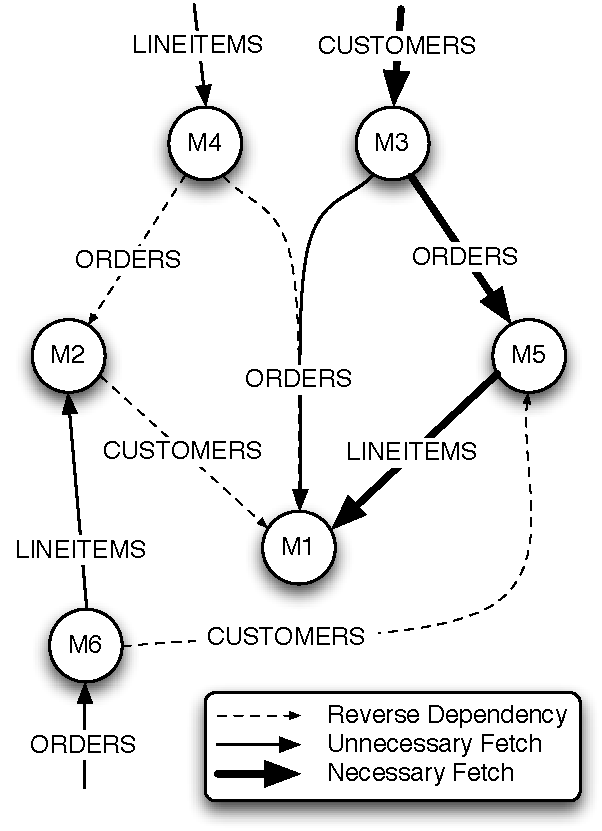
\includegraphics[width=2.5in]{images/q12_graph.pdf}
\caption{Data-flow graph for the example query.
Light and dashed edges can be eliminated.}
\label{fig:dataflow}
\end{center}
\end{figure}


When relations are joined along a key-foreign key relationship,
then we may assume that the transactional databases providing the updates
enforce their consistency. In particular, this means that we cannot use
a foreign key value until it has been inserted as a key; for instance, in
TPC-H, we cannot insert an order with a customer id for which there is
no customer; we first have to insert a suitable customer tuple.
Conversely, we cannot delete a customer until all its dependent orders
have been deleted.\footnote{Suitable code to implement ON DELETE CASCADE
semantics in M3 can be generated by compilation as well, but this is not
covered here because of lack of space.}
Because of lack of space, we only give an illustrative example which
is suggestive of the general algorithm.


\nop{
Thus, given key-foreign key joins, certain M3 statements that our compilation
algorithm produces are superfluous.
Consider a statement
{\tt foreach $\vec{y}$ do $m_2[\vec{x}\vec{y}]$ $\pm$= $t$}
in an on-insert trigger for relation $R$, .

These can be eliminated -- as an
optimization -- by analyzing the data flow graph of the program.
The nodes of this graph are the
map names of the M3 program and where there is an edge labeled $R$ from
node $m_1$ to $m_2$ if there is an M3 statement
{\tt foreach $\cdot$ do $m_2[\cdot]$ $\pm$= $t$} where
$m_1$ appears in $t$ in an insert or delete trigger for relation $R$.
Note that our compilation approach guarantees that this graph is always
acyclic (even if there are self-joins).
} % nop


\begin{example}\em
\label{ex:TPCH-Q12}
Consider the following query on a TPC-H like schema,
which counts the number of LineItems per customer id.
\begin{verbatim}
SELECT   C.cid, SUM(1)
FROM     Customer C, Order O, LineItem L
WHERE    C.cid=O.cid AND O.oid=L.oid
GROUP BY C.cid;
\end{verbatim}
Here, cid is a key for the Customer relation and oid is a key for the
Order relation, but oid is not a key for LineItem.
The compilation algorithm of Section~\ref{sec:compilation-alg} yields the
following insert triggers:
\begin{verbatim}
on insert into Customer(cid, nation) {
  q[cid] += qC[cid];
  foreach oid do qL[cid, oid] += qCL[oid, cid];
  qO1[cid] += 1
}
on insert into Order(oid, cid, ...) {
  q[cid] += qO1[cid]*qO2[oid];
  qC[cid] += qO2[oid];  qL[cid, oid] += qO1[cid];
  qCL[oid, cid] += 1;   qLC[oid, cid] += 1
}
on insert into LineItem(oid, ...) {
  foreach cid do  q[cid] += qL[cid, oid];
  foreach cid do qC[cid] += qLC[oid, cid];
  qO2[oid] += 1
}
\end{verbatim}

Consider the data flow graph for this program, which is shown in
Figure~\ref{fig:dataflow} and which illustrates the dependencies between
maps through updates to certain relations (the edge labels). All M3 statements
contributing dashed edges can be removed because these increments are zero unless a foreign key constraint is violated in the data. For example,
the statement {\tt q[cid] += qC[cid]} in {\tt on insert into Customer}
can be removed because {\tt qC} represents the number of line items for this
customer, and the customer is new. The solid thin lines represent
feasible updates to maps that have become disconnected from the query result
map, and can be eliminated.
The simplification yields the M3 program
\begin{verbatim}
on insert into Customer (cid, ...) { qO1[cid] += 1 }
on insert into Order (oid, cid, ...) {
  qL[cid, oid] += qO1[cid]
}
on insert into LineItem (oid, ...) {
  foreach cid do q[cid] += qL[cid, oid]
}
\end{verbatim}

The delete-triggers are precisely
like the insert-triggers, but with {\tt +=} replaced by {\tt -=}.
\punto
\end{example}





\section{Architecture}
\label{sec:architecture}
\begin{figure}
\begin{center}
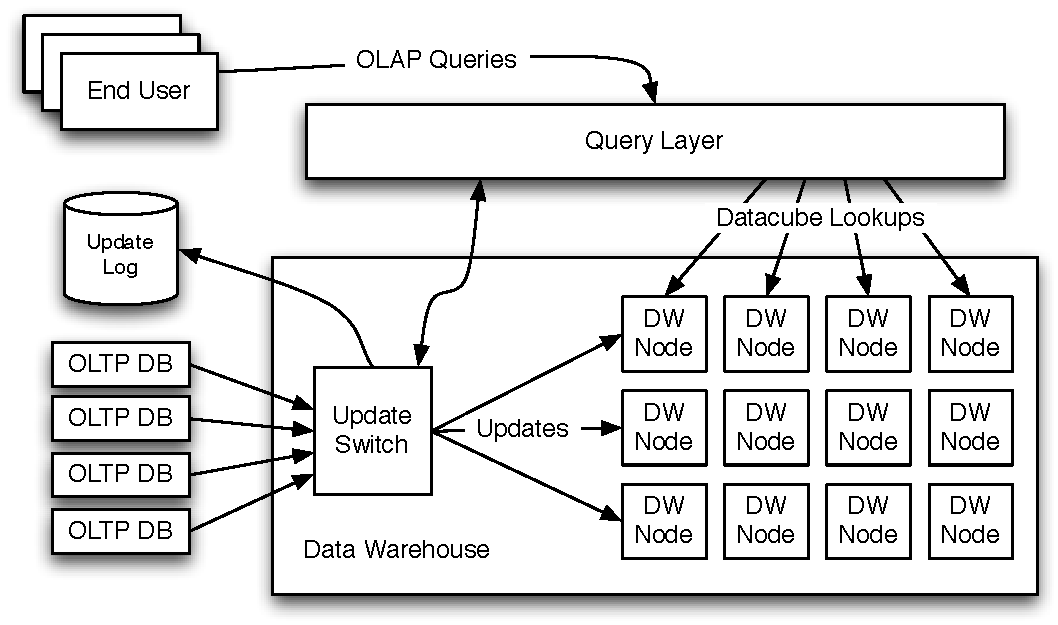
\includegraphics[width=3in]{images/Architecture.pdf}
\caption{Cumulus' architecture.}
\label{fig:arch}
\end{center}
\end{figure}
Cumulus consists of three components: a runtime, a \textit{Query Layer}, and a compiler.  A diagram of this architecture is presented in Figure \ref{fig:arch}.  The warehousing runtime accepts relation updates at a coordinator node called the \textit{Switch}, and distributes their data throughout an array of data warehouse storage nodes, or \textit{DW Nodes}.  Though this paper focuses on a runtime with a centralized switch, we discuss a distributed switch implementation in Section \ref{sec:distswitch}.

Adjacent to the runtime is the \textit{Query Layer}, a component that acts as an intermediary between the end user and the dw nodes.  The query layer accepts roll-up and drill-down queries, translates them into the corresponding set of data warehouse lookups, and executes those queries on the warehouse.

Cumulus' final component is a compiler that guides the behavior of the other three components.  The Cumulus compiler takes schemas for one or more input relations and an arbitrary SQL query as input.  The query is decomposed into a set of subqueries, each representing a join over some subset of the input relations.  Each subquery is materialized into a \textit{map}, that is partitioned across the DW nodes.  

Based on these subqueries, the compiler generates a series of \textit{update rules} that translate changes in the input relations to map deltas.  These update rules take the form:
$$+R(x_1, x_2, x_3, \ldots)\ :\ Map\ K[\ldots]\ += Expression$$
That is, when the tuple $(x_1, x_2, x_3, \ldots)$ is inserted into input relation $R$, adjust the target map $K$ by the indicated arithmetic expression over constants, variables ($x_n$), or the contents of other maps.  
 
It is possible for an update rule to modify an an entire cross section of a map.  Such updates are expressed via variables in the update rule not bound to one of the input parameters.  We refer to these as loop variables.  A loop variable occurs exactly twice in an update rule, once as a key in the target map, and once as an key for a map in the expression.  Thus an update rule with loop variables behaves as if it were a set of parallel updates; every update corresponds to one possible valuation of all loop variables selected from the domains of the map they index into.

When a tuple is added to or removed from an input relation, the Switch composes a set of messages parametrized on the tuple's contents and dispatches them into the data warehouse as a sequence of map reads and writes.  Nodes being read from accept and process the requests and forward the responses to the appropriate writers.  We refer to this entire sequence of operations as an update.

\begin{example}
One of the rules the compiler generates for updates to the lineitems table in the example datacube is
{\footnotesize
\begin{eqnarray*}
+lineitems(l\_oid,lateship,latedeliver,shipmode) : \\
Map\ 1[shipmode,latecommit,lateship,spriority,\\ opriority,l\_oid,cid,nation] \\
 += Map\ 5[cid,nation,l\_oid,opriority,spriority]
\end{eqnarray*}}
\noindent Here, Map 1 represents the query output $count(*)$, while Map 5 represents the natural join $customers \bowtie orders$\footnote{Map 5 actually represents the $count(*)$ of the join, grouped by all columns.  However, because $cid$ and $oid$ are keys for each input table, the count is binary; Each entry in Map 5 is either 0 or 1.  It is also possible to treat Map 5 as a map from $(cid,oid)$ to $\{(nation, opriority, spriority)\}$. }.  Note that the variables $cid$, $nation$, $opriority$, and $spriority$ do not appear in the input tuple.  These variables are treated as loop variables; an entire cross-section of Map 1 will be updated by the values stored in the corresponding portion of Map 5.  

The update corresponding to this rule is coordinated by a subset of nodes that store partitions of Map 1.  Each node coordinates updates only for those partitions it stores locally.  Simultaneously, read requests are dispatched by the switch to a subset of the nodes managing partitions of Map 5, and the responses are forwarded to the appropriate Map 1 nodes.  
\end{example}

\subsection{Anatomy of an Update}

\begin{figure}
\begin{center}
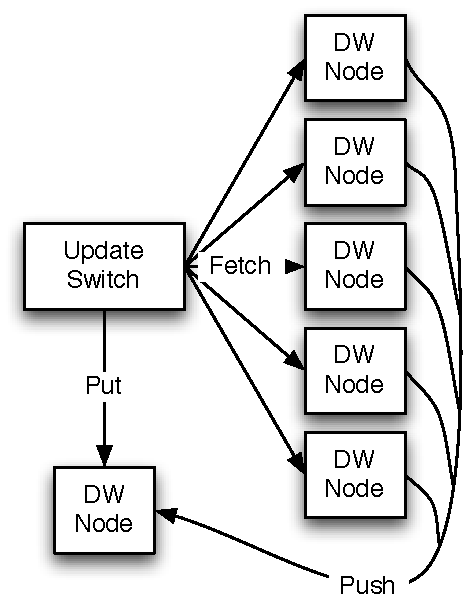
\includegraphics[width=1.5in]{images/UpdateStep.pdf}
\caption{Information flow during one map update.}
\label{fig:updatestep}
\end{center}
\end{figure}

A map update begins at the Switch when an input table is modified.  Each input table is associated with one or more triggers, each requiring a write to some range of map values and zero or more reads from different maps.  For each trigger, the Switch identifies and sends a PUT message to each DW Node managing a map being written to.  Additionally, the Switch identifies all DW Nodes managing maps that will be read from and sends a FETCH message to them, requesting the desired map values.  Finally, if required (i.e., if Cumulus is being used standalone, without an underlying database), the switch can log the update to disk for persistence.

The nodes receiving a FETCH request perform the appropriate reads and send their responses to the PUT nodes in a PUSH message.  Upon receipt of all necessary PUSH messages, the PUT nodes compute the update expression and modify the affected maps.  An illustration of the complete message-passing process is presented in Figure \ref{fig:updatestep}.  

\subsubsection{Trigger Dispatch}
Maps are partitioned along dimensional axes when they grow beyond the capacity of a single node, akin to the partitioning done in grid files\cite{318586}.  To streamline the dispatch of messages to component nodes, the switch pre-generates a spatial index for each template, similar to the grid file directory.  Every entry in the spatial index contains a set of PUT and FETCH messages.  When the template is triggered, the tuple's values are used to index into the spatial index and the corresponding messages are parametrized and sent.  The algorithm for generating the spatial index is presented in Figure \ref{alg:dispatch}.

\begin{figure}
\begin{algorithmic}[1]
\STATE $Msgs \leftarrow \emptyset$
\FORALL{Update $U \in$ Trigger}
	\STATE Region $Reg = \pi_{U.target.loop\_vars} \left(index(U.target\_map)\right)$
	\FORALL{Partition $\{P | P\in U.target\_map \wedge (P \cap Reg \neq \emptyset)\}$}
		\STATE $Reads = \emptyset$
		\FORALL{Ref $R \in get\_map\_refs(U.expression)$}
			\STATE $RReg \leftarrow \pi_{R.loop\_vars} P$
			\STATE $RPart \leftarrow \{RP | RP\in R.map \wedge (RP \cap RReg \neq \emptyset)\}$
			\STATE $Reads \leftarrow Reads \cup \{(ReadP.node, R)\}$
		\ENDFOR
		\STATE $Reads \leftarrow group\_by\_node(Reads)$
		\STATE $Msgs \leftarrow put(U, P, Reads.size)$
		\FORALL{$($Node $N, \{$Ref $R\}) \in Reads$}
		  \STATE // PUSH results to $P.node$
			\STATE $Msgs \leftarrow fetch(N, \{R\}, P.node)$
		\ENDFOR
	\ENDFOR
\ENDFOR
\end{algorithmic}
\caption{The Switch's trigger dispatch algorithm}
\label{alg:dispatch}
\end{figure}

Looping updates require the Switch to match corresponding read and write partitions.  The correspondence is obtained by identifying intersections between partitions of the target map that are affected by the update, and those of each map in the update expression.  This is equivalent to a join over components of the spatial index stored at the Switch.  Loop-free updates are a special case of this, where only one partition is required from each map.  The trigger dispatch algorithm is shown in Figure \ref{alg:dispatch}.

\subsubsection{Get Collation}

FETCH responses, or PUSH messages for an update are sent to the node managing the partition being updated.  Having received the number of FETCH messages sent by the switch with the PUT message, the destination node can buffer PUSH messages until all have arrived.  At this point, if the update is loop-free, the destination node simply uses the contents of the PUSH messages to evaluate the update expression.

\begin{figure}
\begin{algorithmic}[1]
\STATE Given: Update $U$
\FORALL{Ref $R \in U.expression$}
	\STATE $Inputs \leftarrow Inputs \cup (R, \emptyset)$
\ENDFOR
\FORALL{$($Ref $InR,$ Value $V) \in \cup(msg_{PUSH})$}
	\FORALL{$(R, Table) \in Inputs$}
		\IF{$check\_match(InR, R)$}
			\STATE $Table \leftarrow Table \cup (InR.keys, V)$
		\ENDIF
	\ENDFOR
\ENDFOR
\FORALL{$(K,\{V\}) \in $ JOIN $ (Keys, Val) \in Inputs$}
	\STATE $Target = bind\_vars(U.target \leftarrow Keys)$
	\STATE $apply(Target, bind\_vars(U.expression \leftarrow \{V\}))$
\ENDFOR
\end{algorithmic}
\caption{The DW Node's collation algorithm}
\label{alg:collation}
\end{figure}

If the update requires a loop, the destination node must do some processing.  The node first generates a set of tables, one for each map reference in the update expression.  Arriving map values populate tables that correspond to any map reference matching the value's keys, where loop variables act as wildcards.  When all values have been received, the destination node computes the natural join of all of the generated tables, effectively producing one update value for every assigned value in the domain of all of the loop variables.  The loop-free update is a special case of this where each generated table contains only one row.  The collation algorithm is shown in Figure \ref{alg:collation}

\subsection{Update Consistency and Garbage Collection}

Cumulus' delta-encoding approach allows it to be agnostic to the order in which it processes input tuples.  However, this flexibility requires that an update's effect on the warehouse be logically atomic.  Atomicity is of particular importance, since the set of update rules triggered by a given update switch typically span the breadth of the data-dependency graph; Updates to any input relation typically have at least one read to a map updated by every other relation.

As the clearinghouse for updates, the Switch presents an ideal point for generating a total ordering over all tuples to be inserted into the warehouse.  The Switch maintains a version number for each node, incremented on every PUT dispatched to the node hosting it.  FETCHes sent to that node are tagged with the version number of the last PUT sent to the node, while PUTs are dependent on the completion of the prior PUT.

Data warehouse nodes ensure consistent evaluation of updates by buffering PUT requests received out of order, or prior to the completion of an earlier PUT request.  Similarly, FETCH requests for a particular version are buffered until the corresponding PUT request has completed, if it hasn't already done so.

Periodically, the switch queries each node for the completion status of pending PUT requests.  For each node, it computes the lowest FETCH version number for a read associated with an incomplete PUT request.  The Switch then disseminates these version numbers throughout the warehouse with a COMMIT message.  When a node receives a COMMIT, it snapshots its maps by discarding all updates for values that were overwritten before the commit version.

\section{Compilation}
\label{sec:compilation}

\subsection{Update Rules}
- Translating SQL into Update Rules

- Update DAGs/Data flow graphs

- Exploiting Foreign Keys

- Cascading Map Rejection

\begin{figure}
\begin{center}
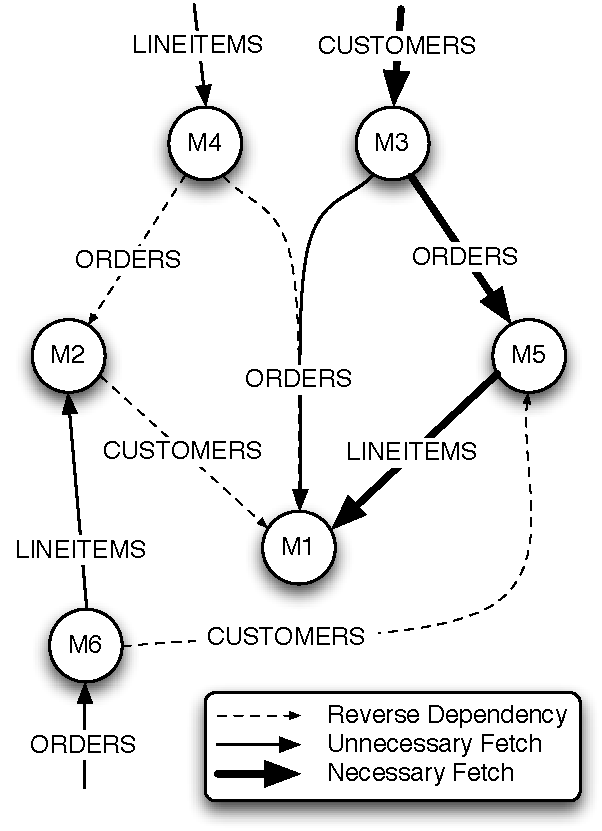
\includegraphics[width=2.5in]{images/q12_graph.pdf}
\caption{Data-flow graph for the example query.  Light and dashed edges can be optimized out, given cascading delete foreign key constraints.}
\label{fig:dataflow}
\end{center}
\end{figure}

\subsection{Layout}
How do we partition data (the layout)?  Where do various bits of code get executed live?  What kind of runtime analytics do we need to collect to manage the data layout on the fly? 


\section{Experiments}
\label{sec:experiments}

\section{Optimizations}
\label{sec:optimizations}

\subsection{Distributing the Switch}
\label{sec:distswitch}
The role of the switch is to provide a synchronization mechanism for the updates.  Specifically, the delta encoding approach used by the update rules requires that all update rules be applied to a consistent snapshot of the maps.  The current implementation of Cumulus performs this synchronization at a single node.  However, limiting the switch to only one node creates a scaling bottleneck.  

Despite the cloud computing mantra of rejecting consistency, this application requires it.  Complex locking protocols have poor scaling performance, so a simpler, lock-free protocol is required.  We achieve this goal by introducing the notion of \textit{pipeline scheduling}.  Pipeline scheduling exploits the acyclicity of compiler-generated data-flow graphs to allow nodes to correctly interleave and process update rules with only limited network overhead and processing latency.

\subsection{Pipeline Scheduling}
Loose clock synchronization between nodes is assumed, and allows time to be partitioned into a sequence of numbered ticks, each lasting on the order of seconds.  When a set of updates is triggered, a switch node sends tentative put requests to all participating nodes.  These nodes respond with their current tick counter, and the switch forwards the maximum returned tick to all nodes.

The updates are considered to have been posted at the maximum returned tick.  However processing is deferred for a number of ticks equal to the depth of the map being updated.  The result is a data-flow process resembling a parallelized CPU pipeline.

During a given tick, all updates scheduled for processing are evaluated.  Once all updates scheduled for the tick have completed, the node responds to FETCH requests for the tick with PUSH messages.  Recall that each edge in the data flow graph represents a FETCH request for a specific update.  The difference in depth between the edge's ends is the number of ticks in advance of the PUT that the response is sent.  

For example, in Figure \ref{fig:dataflow} without removing any edges, $Depth(M1) = 2$, $Depth(M2) = 1$, and $Depth(M4) = 0$.  Updates to map $M1$ scheduled for processing during tick 4 would receive data from map $M2$ during tick 3, and from map $M1$ during tick 2.

%\subsection{Synchronizing Ticks}
%Ensuring that nodes are operating on the same tick poses two challenges.  First, the nodes must 
%
%Clock tick synchronization requires two pieces of functionality: Asserting 
%
%Loose clock tick synchronization requires two stages.  
%
%is achieved through a cascading gossip protocol.
%
%
%\subsection{Distributed Queries}
%

\section{Conclusions}
\label{sec:conclusions}

\bibliographystyle{abbrv}
\bibliography{main}




%\begin{figure}
%\begin{center}
%\begin{itemize}
%\item Middleware
%\begin{itemize}
%\item Query(Query) 
%\end{itemize}
%
%\item Warehouse Nodes
%\begin{itemize}
%\item Get(\{Entry\}, Version)
%\item Fetch(\{Entry\}, Version, Destination)
%\item Push(\{(Entry, Value)\}, Version)
%\item Put(Template, \{Params\}, Version [, Fetches])
%\end{itemize}
%
%\item Switch
%\begin{itemize}
%\item update(Relation, \{Params\})
%\end{itemize}
%
%\end{itemize}
%\caption{Cumulus' API}
%\label{fig:api}
%\end{center}
%\end{figure}

\end{document}  
